\def \makebasiclayers{
    \section{Một số lớp cơ bản trong các mô hình deep learning}
    Trong suốt quá trình phát triển của các mô hình deep learning\index{deep learning}, có rất nhiều các layer được xây dựng và phát triển với những mục đích khác nhau nhằm khai thác một cách hiệu quả nhất các đặc trưng của dữ liệu. Tuy nhiên, trong khuôn khổ của đồ án tốt nghiệp, ta chỉ nghiên cứu những layer xuất hiện trong các mô hình được giới thiệu ở phần sau của đồ án.

    \subsection{Lớp fully-connected}
    Mỗi hidden layer \index{hidden layer} trong một mạng nơ ron thông thường được gọi là một lớp fully-connected \index{fully-connected} (fully-connected layer\index{fully-connected layer}). Lớp này được gọi như vậy bởi vì với mỗi nơ ron trong fully-connected layer được kết nối với tất cả các nơ ron \index{nơ ron} trong fully-connected layer trước nó. Cả mô hình được gọi là fully-connected neural network \index{fully-connected neural network} (FCN\index{FCN}) hoặc multilayer perceptron \index{multilayer perceptron} (MLP\index{MLP}).

    \begin{figure}[H]
    \centering
    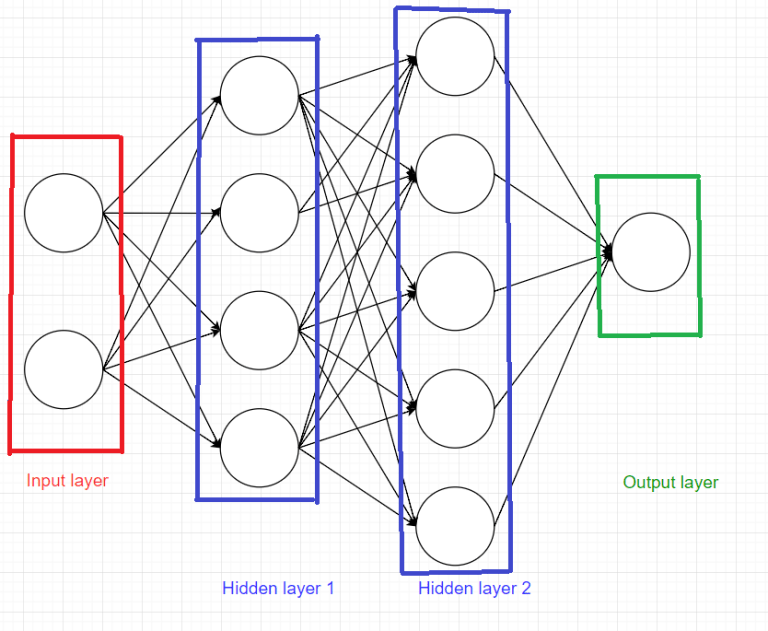
\includegraphics[width=7cm] {images/neural_net.png}
    \caption{Kiến trúc của mạng nơ ron \index{mang nơ ron} (neural network\index{neural network}) thông thường (Nguồn: nttuan8.com)}
    \label{fig:neural_net}
    \end{figure}
    
    \subsection{Lớp convolution}
    Phép tính tích chập \index{tích chập} (convolution\index{convolution}) được dùng trong lớp convolution (convolution layer\index{convolution layer}) giúp giải quyết vấn đề về số lượng trọng số của mô hình (so với fully-connected layer) và giúp lấy được các đặc trưng của dữ liệu có tính không gian (ảnh, video ...) một cách hiệu quả.

    \begin{figure}[H]
    \centering
    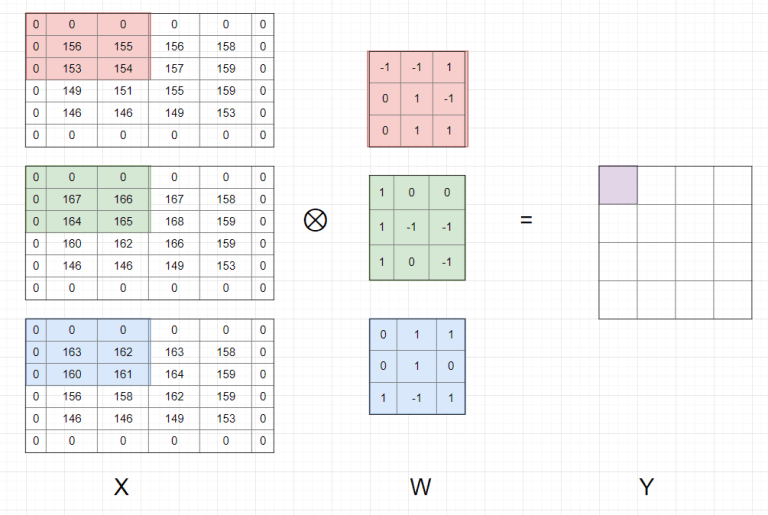
\includegraphics[width=12cm] {images/conv.png}
    \caption{Phép tính tích chập trong mỗi convolution layer (Nguồn: nttuan8.com)}
    \label{fig:conv_layer}
    \end{figure}

    \noindent Một số khái niệm cơ bản đối với lớp convolution:
    \begin{itemize}[leftmargin=0cm,itemindent=.5cm,labelwidth=\itemindent,labelsep=0cm,align=left]
        \item Kernel: Là một ma trận có kích thước nhỏ (thường là 1x1, 3x3, 7x7, ...) hoạt động như một bộ lọc chứa các trọng số cần thiết trong việc lấy ra các đặc trưng của dữ liệu. Với mỗi kernel khác nhau, mô hình sẽ học được những đặc trưng khác nhau của ảnh, nên trong mỗi convolutional layer ta sẽ dùng nhiều kernel\index{kernel} để học được nhiều thuộc tính của ảnh.
        \item Features map: Là kết quả của dữ liệu sau khi đi qua một kernel, chứa các đặc trưng nổi bật đại diện cho dữ liệu và là nguyên liệu sử dụng cho các bài toán khác nhau.
        \item Stride: Là bước nhảy của kernel. Nếu stride\index{stride} bằng 1, kernel sẽ di chuyển tuần tự qua từng vị trí của features map\index{features map}. Nếu stride lớn hơn 1, kernel sẽ bỏ qua một số vị trí trên features map.
        \item Padding: Là phép thêm các giá trị vào features map trước khi thực hiện phép convolution, điều này giúp cho features map đầu vào và features map đầu ra có kích thước chiều dài và chiều rộng giống nhau. Một số phương pháp padding\index{padding} có thể kể đến như: constant padding\index{constant padding} - padding với một giá trị không đổi (thường là 0), reflection padding\index{reflection padding} - padding với các giá trị đối xứng trong features map.
    \end{itemize}
    
    \begin{figure}[H]
    \centering
    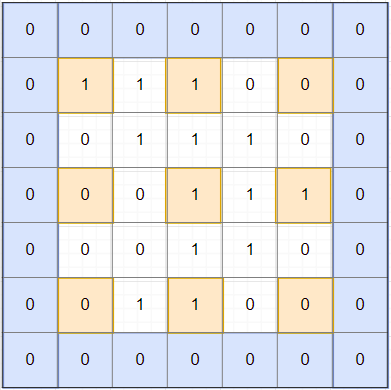
\includegraphics[width=5cm] {images/stride_pad.png}
    \hspace{1.5cm}
    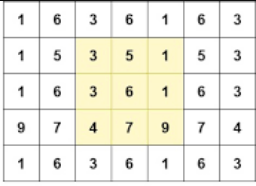
\includegraphics[width=5cm] {images/padding_reflection.png}
    \caption{(trái) Padding với giá trị 0 không đổi và stride bằng 1, (phải) Padding với các giá trị đối xứng (Nguồn: nttuan8.com, machinecurve.com)}
    \label{fig:stride_pad}
    \end{figure}
    
    \subsection{Lớp average pooling}
    Lớp pooling\index{pooling} nói chung thường được dùng giữa các lớp convolution, với mục tiêu để giảm kích thước của dữ liệu (chiều dài và chiều rộng đối với dữ liệu ảnh) nhưng vẫn giữ được các đặc trưng quan trọng. Lớp pooling giúp giảm số lượng tính toán trong quá trình luyện mô hình.\\
    Lớp average pooling\index{average pooling} (average pooling layer\index{average pooling layer}) lấy trung bình của các giá trị trên features map theo từng kích thước của kernel pooling\index{kernel pooling}.
    \begin{figure}[H]
    \centering
    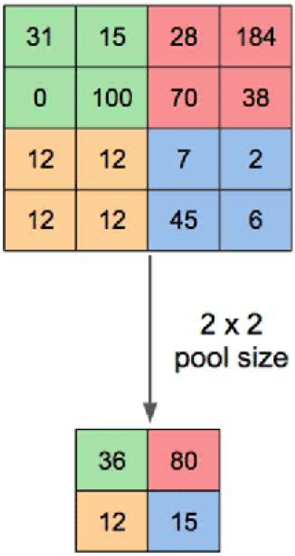
\includegraphics[width=3cm] {images/avg_pool.png}
    \caption{Phép average pooling trong average pooling layer (Nguồn: medium.com)}
    \label{fig:avg_pool}
    \end{figure}
    \noindent Bên cạnh các layer pooling thông thường giúp giảm kích thước của features map, lớp global average pooling\index{global average pooling} (GAP\index{GAP}) giúp giảm số chiều của features map bằng cách lấy trung bình tất cả các giá trị tại mỗi channel\index{channel} của features map.
    \begin{figure}[H]
    \centering
    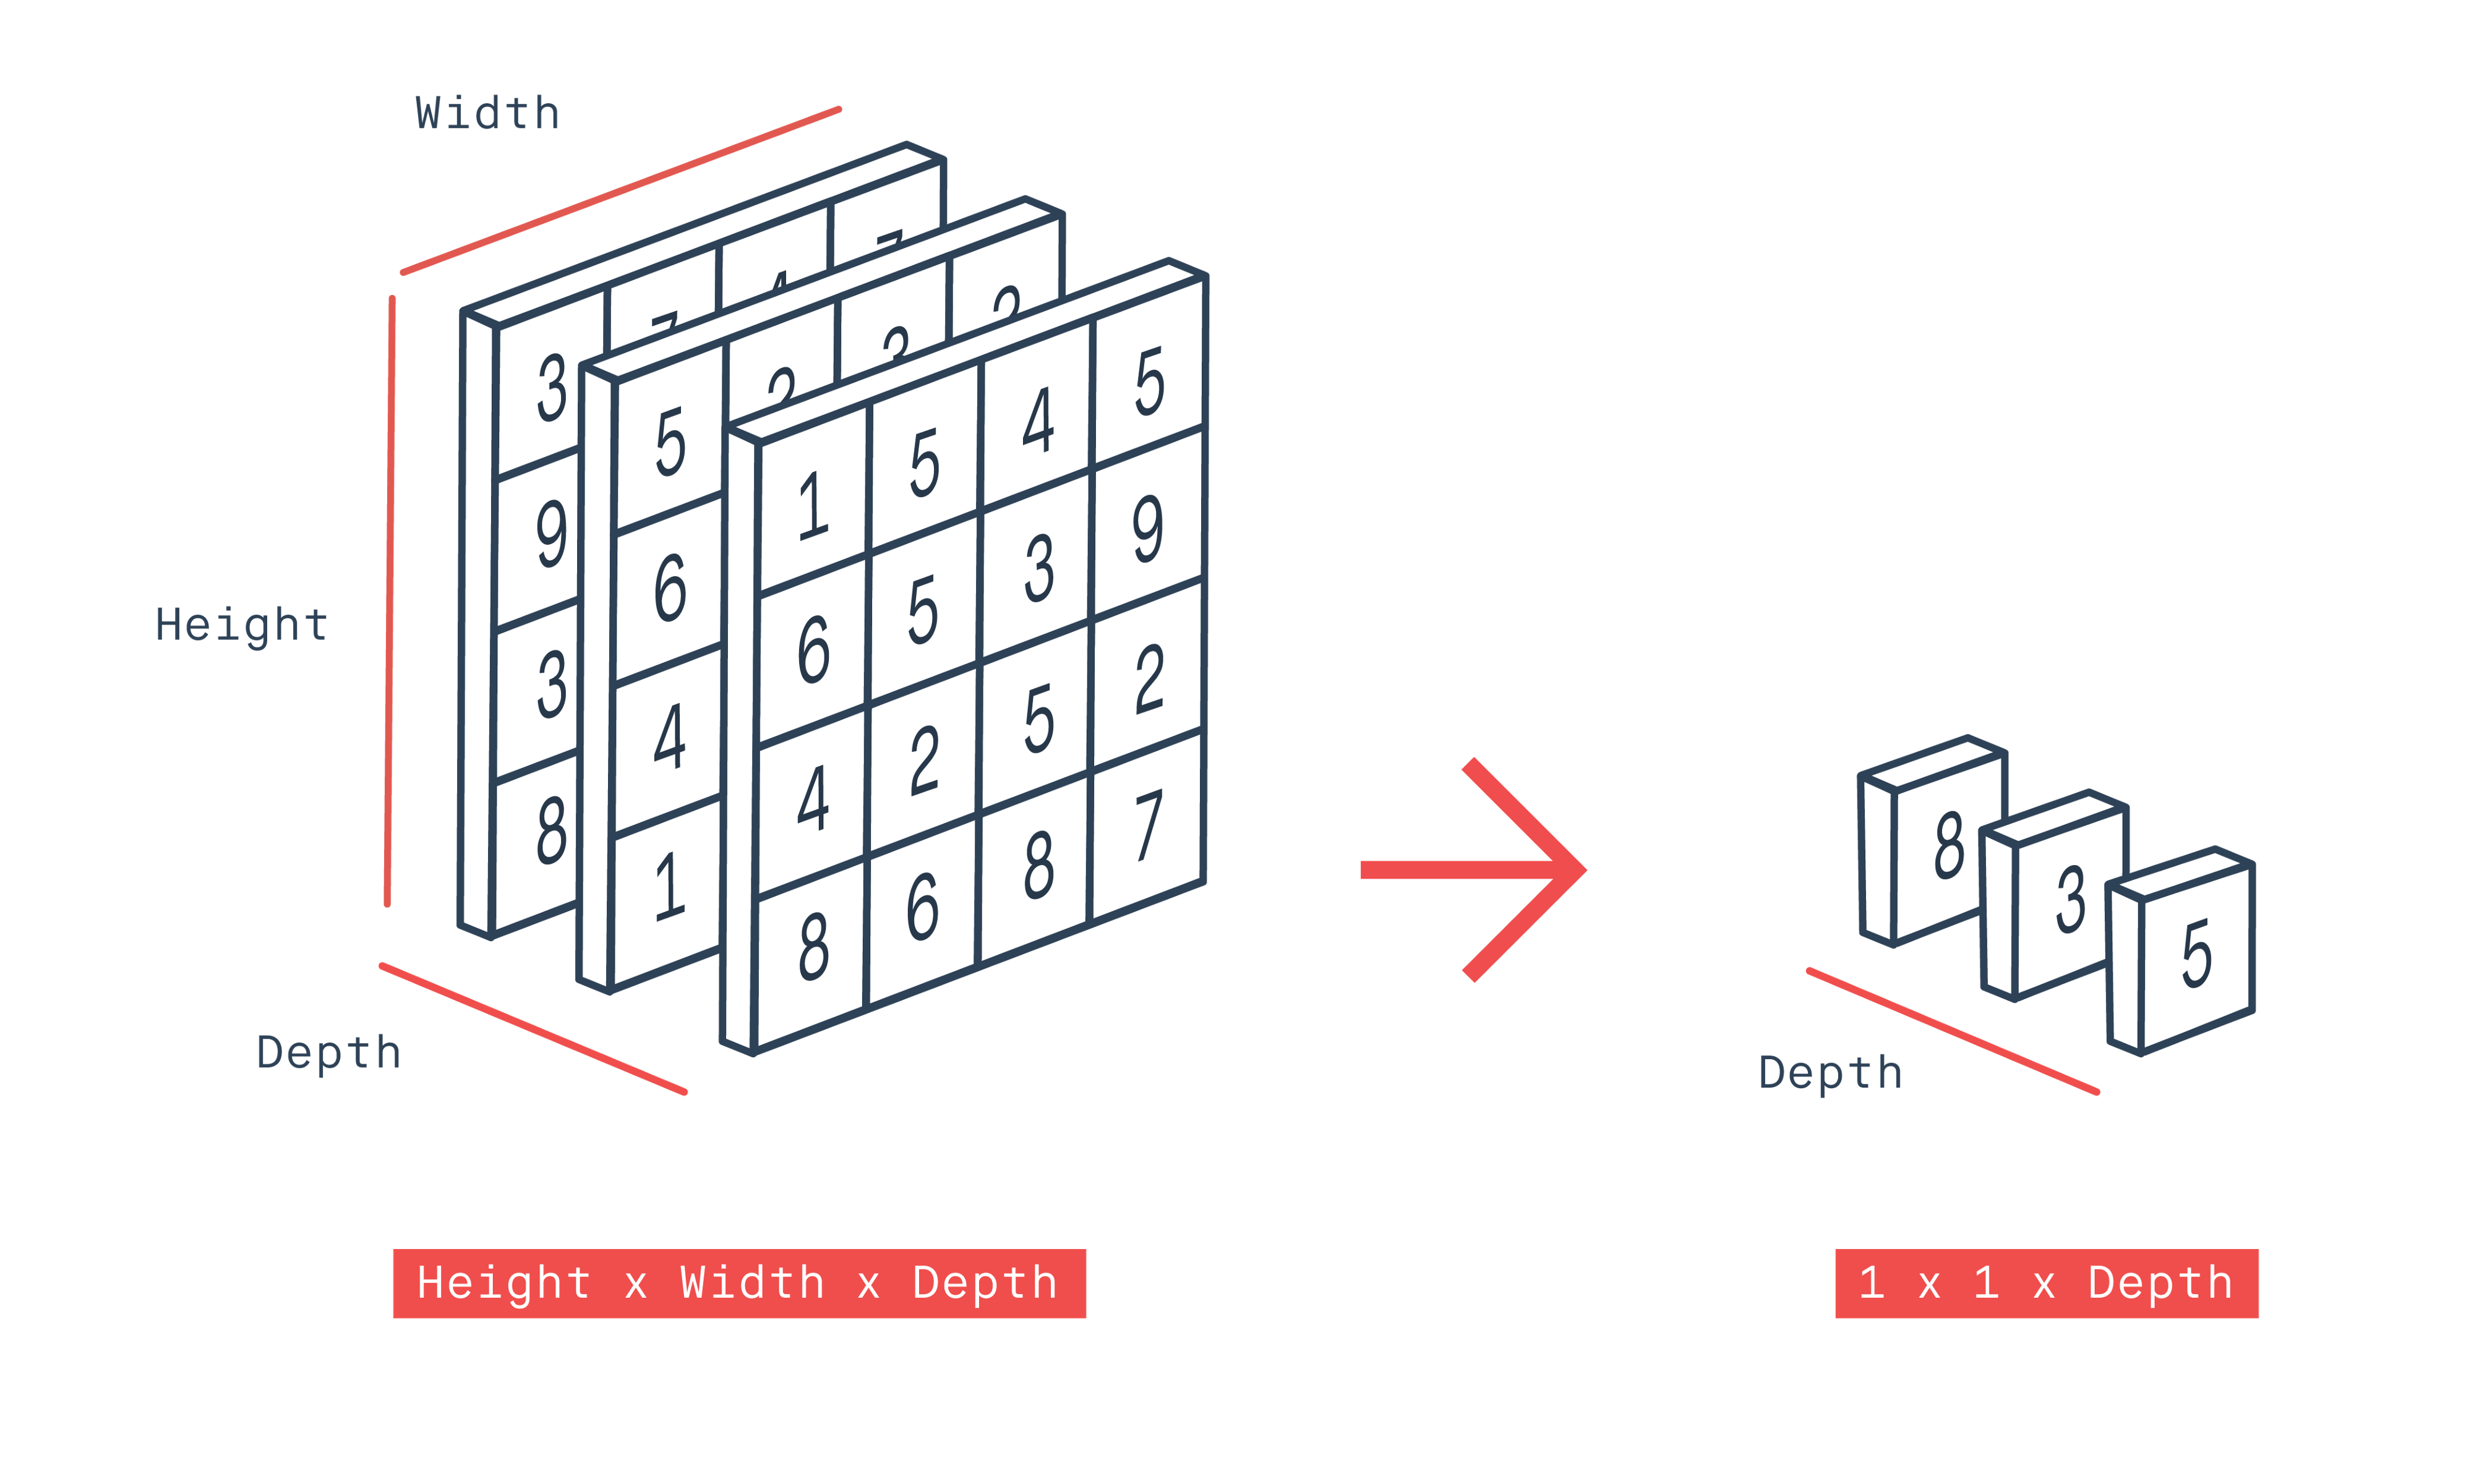
\includegraphics[width=8cm] {images/gap.png}
    \caption{Phép average pooling trong global average pooling layer\index{global average pooling layer} (Nguồn: medium.com)}
    \label{fig:gap}
    \end{figure}

    \subsection{Lớp sigmoid}
    Sigmoid là một hàm kích hoạt\index{hàm kích hoạt} khiến cho các giá trị đầu ra trở nên phi tuyến tính. Giá trị đầu ra của sigmoid\index{sigmoid} nằm trong khoảng [0, 1]. Từ đó, ta có thể coi như giá trị này mang tính chất về xác suất (gần 1 nghĩa là xác suất lớn và gần 0 nghĩa là xác suất nhỏ).\\
    Sigmoid thường được sử dụng trong layer cuối cùng để giải các bài toán phân lớp\index{bài toán phân lớp} như binary classification\index{binary classification}, multi label classification\index{multi label classification} ...

    \begin{figure}[H]
    \centering
    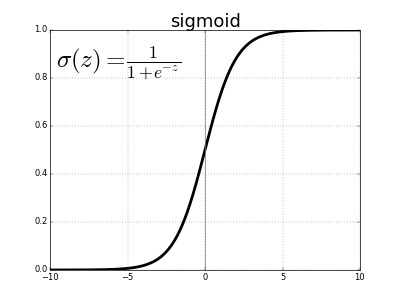
\includegraphics[width=6cm] {images/sigmoid.jpeg}
    \caption{Hàm và đồ thị của sigmoid (Nguồn: quora.com)}
    \label{fig:sigmoid}
    \end{figure}

    \subsection{Lớp ReLU và lớp Leaky ReLU}
    \index{ReLU}ReLU, tên đầy đủ là Rectified Linear Unit\index{Rectified Linear Unit}, là một hàm kích hoạt khiến cho các giá trị đầu ra trở nên phi tuyến tính\index{phi tuyến tính}. Giá trị đầu ra của ReLU nằm trong khoảng [0, +$\infty$].\\
    Hầu hết, trong các mô hình liên quan tới bài toán computer vision\index{computer vision}, ta sử dụng ReLU layer phía sau các convolution layer và normalization layer\index{normalization layer} bởi vì nó giúp giảm thiểu các vấn đề liên quen đến đạo hàm và cải thiện tốt tốc độ hội tụ của mô hình. Tuy nhiên, ReLU cũng có một số điểm yếu như: bất đối xứng tại điểm 0 và không có đạo hàm tại các điểm nhỏ hơn 0 mặc dù có thể đạo hàm tại bất kỳ mọi điểm nào khác.\\
    Một số biến thể của ReLU có thể kể đến là: Softplus\index{Softplus} (SmoothReLU\index{SmoothReLU}), Noisy ReLU\index{Noisy ReLU}, Leaky ReLU\index{Leaky ReLU}, Parametric ReLU\index{Parametric ReLU} và ExponentialReLU\index{ExponentialReLU} (ELU\index{ELU}).
    
    \begin{figure}[H]
    \centering
    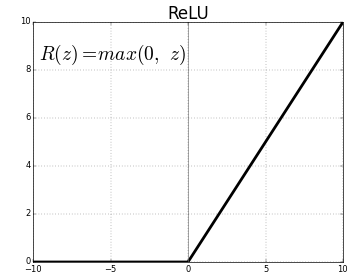
\includegraphics[width=6cm] {images/relu.png}
    \caption{Hàm và đồ thị của ReLU (Nguồn: medium.com)}
    \label{fig:conv_layer}
    \end{figure}

    Nhằm cải thiện vấn đề mất mát đạo hàm tại các giá trị nhỏ hơn 0 của hàm ReLU, hàm Leaky ReLU đã ra đời. Đồ thị của Leaky ReLU có độ dốc nhỏ với các phần tớ nhỏ hơn không, giúp đạo hàm tại điểm nhỏ hơn 0 tồn tại.
    
    \begin{figure}[H]
    \centering
    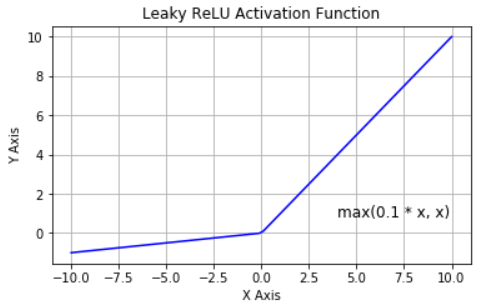
\includegraphics[width=7cm] {images/leaky.png}
    \caption{Hàm và đồ thị của Leaky ReLU (Nguồn: researchgate.net)}
    \label{fig:conv_layer}
    \end{figure}
    
    \subsection{Lớp instance normalization}
    Lớp instance normalization\index{instance normalization} (instance normalization layer\index{instance normalization layer}) được đề xuất trong việc giải quyết bài toán chuyển đổi style của ảnh (style transfer)\index{style transfer}. Năm 2016, Ulyanov và các cộng sự lần đầu thử nghiệm việc sử dụng instance normalization trong mô hình giải bài toán chuyển đổi style của ảnh (style transfer) và đạt được kết quả vượt trội hơn so với mô hình tương tự sử dụng batch normalization\index{batch normalization}. Hơn nữa, một điểm mạnh của instance normalization so với batch normalization là sự đồng nhất giữa quá trình huấn luyện và kiểm tra mô hình trong khi các trọng số trong batch normalization layer là không đồng nhất trong quá trình huấn luyện và kiểm tra.
    \begin{align}
    \textrm{IN}(x)= \gamma\left(\frac{x-\mu(x)}{\sigma(x)}\right)+\beta  ,
    \end{align}
    \begin{align}
    \mu_{nc}(x) = \frac{1}{HW}\sum_{h=1}^{H}\sum_{w=1}^{W}x_{nchw}  ,
    \end{align}
    \begin{align}
    \sigma_{nc}(x) = \sqrt{\frac{1}{HW}\sum_{h=1}^{H}\sum_{w=1}^{W}(x_{nchw} - \mu_{nc}(x))^{2} + \epsilon}  ,
    \end{align}
	\noindent trong đó:
	\begin{itemize}[leftmargin=0cm,itemindent=.5cm,labelwidth=\itemindent,labelsep=0cm,align=left]
        \item $x$: features map đầu ra của layer convolution trước đó.
        \item $\textrm{IN}(x)$: features map đầu ra của layer convolution trước đó.
        \item $\mu(x)$ và $\mu_{nc}(x)$: mean theo từng channel của từng features map đầu vào.
        \item $\sigma(x)$ và $\sigma_{nc}(x)$: standard deviation theo từng channel của từng features map đầu vào.
        \item $\gamma$: là giá trị trọng số cần được luyện của instance normalization layer.
        \item $\beta$: là giá trị trọng số cần được luyện của instance normalization layer.
        \item H: là chiều rộng kích thước features map đầu vào.
        \item W: là chiều dài kích thước features map đầu vào.
    \end{itemize}

    \subsection{Lớp adaptive instance normalization}
    Là một phiên bản mở rộng của instance normalization, được giới thiệu vào năm 2017, adaptive instance normalization\index{adaptive instance normalization} (gọi tắt là AdaIN\index{AdaIN}) \cite{adain} là một ý tưởng thú vị trong việc giải bài toán chuyển đổi style của ảnh (style transfer). AdaIN thay các tham số của biến đổi affine trong phép normalize thông thường bằng các giá trị đại diện cho phân phối xác suất của style cần biến đổi. Do đó, khác với các lớp normalization khác, AdaIN không có trọng số nào cần phải học trong quá trình luyện mô hình.
    \begin{align}
    \textrm{AdaIN}(x, y)= \sigma(y)\left(\frac{x-\mu(x)}{\sigma(x)}\right)+\mu(y)
    \end{align}
	\noindent trong đó:
	\begin{itemize}[leftmargin=0cm,itemindent=.5cm,labelwidth=\itemindent,labelsep=0cm,align=left]
        \item x: features map đầu ra của layer convolution trước đó.
        \item y: features map của style mà ta muốn chuyển đổi tới.
        \item $\mu(x)$: mean theo chiều channel của features map đầu vào.
        \item $\sigma(x)$: standard deviation theo chiều channel của features map đầu vào.
        \item $\mu(y)$: là giá trị mean của style đầu vào.
        \item $\sigma(y)$: là giá trị standard deviation của style đầu vào.
    \end{itemize}

    \subsection{Lớp layer normalization}
    Lớp layer normalization\index{layer normalization} được để xuất lần đầu nhằm giải quyết vấn đề liên quan đến việc các mô hình sử dụng batch normalization sẽ không đạt kết quả tốt nếu như batch size\index{batch size} nhỏ. Trong bài báo đề xuất, tác giả giới thiệu việc sử dụng layer normalization trong mô hình MLP và recurrent neural network\index{recurrent neural network} (RNN\index{RNN}), tuy nhiên, sau này, các mô hình convolution neural network\index{convolution neural network} (CNN\index{CNN}) cũng sử dụng layer normalization như một cách kiểm soát mối tương quan thống kê giữa các channel trong một features map.
    \begin{align}
    \mu^l = \frac{1}{H}\sum_{i = 1}^H  \alpha^l_i
    \qquad
    \sigma^l = \sqrt{\frac{1}{H}\sum_{i = 1}^H  \left( \alpha^l_i  - \mu^l \right)^2}
    \end{align}
	\noindent trong đó:
	\begin{itemize}[leftmargin=0cm,itemindent=.5cm,labelwidth=\itemindent,labelsep=0cm,align=left]
        \item $\alpha^l_i$: giá trị của nơ ron thứ i trong layer l.
        \item $\mu^l$: mean\index{mean} của các nơ ron trong cùng một layer l.
        \item $\sigma^l$: standard deviation\index{standard deviation} của các nơ ron trong cùng một layer l.
        \item $H$: số nơ ron trong layer l.
    \end{itemize}
    \subsection{Lớp nearest neighbors }
    Lớp nearest neighbors\index{nearest neighbors} (nearest neighbors layer\index{nearest neighbors layer}) dựa trên phép nearest neighbors là một trong những layer rất đơn giản trong việc tăng kích thước của ảnh. Chi tiết về lớp nearest neighbors được minh hoạ trong hình \ref{fig:nn}.

    \begin{figure}[H]
    \centering
    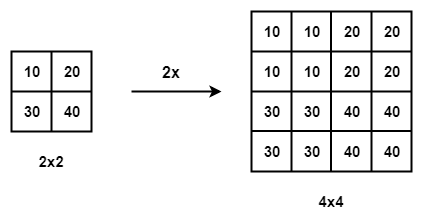
\includegraphics[width=7cm] {images/nn.png}
    \caption{Phép nearest neighbors trong Nearest neighbors layer (Nguồn: theailearner.com)}
    \label{fig:nn}
    \end{figure}

    \subsection{Khối residual}
    Khối residual\index{residual} (residual block\index{residual block}) lần đầu được xuất hiện trong kiến trúc của ResNet\index{ResNet} \cite{resnet} với mục tiêu giảm vấn đề về mất mát đạo hàm, giúp các mô hình deep learning có thể phức tạp hơn và sâu hơn. Điểm đặc biệt trong kiến trúc của một residual block chính là đường nối skip connection\index{skip connection} giúp các thông tin nguyên bản từ đầu vào của block có thể được truyền tới đầu ra của block.

    \begin{figure}[H]
    \centering
    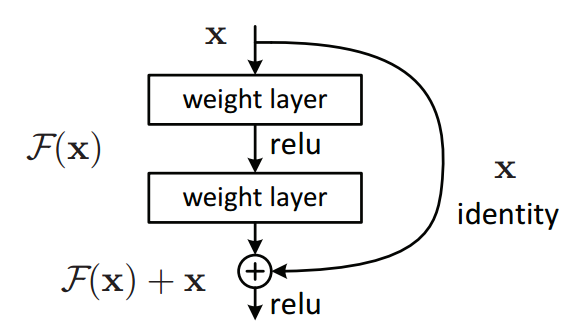
\includegraphics[width=7.5cm] {images/residual.png}
    \caption{Kiến trúc của một khối residual (Nguồn: medium.com)}
    \label{fig:residual}
    \end{figure}
}